\PassOptionsToPackage{unicode=true}{hyperref} % options for packages loaded elsewhere
\PassOptionsToPackage{hyphens}{url}
%
\documentclass[]{book}
\usepackage{lmodern}
\usepackage{amssymb,amsmath}
\usepackage{ifxetex,ifluatex}
\usepackage{fixltx2e} % provides \textsubscript
\ifnum 0\ifxetex 1\fi\ifluatex 1\fi=0 % if pdftex
  \usepackage[T1]{fontenc}
  \usepackage[utf8]{inputenc}
  \usepackage{textcomp} % provides euro and other symbols
\else % if luatex or xelatex
  \usepackage{unicode-math}
  \defaultfontfeatures{Ligatures=TeX,Scale=MatchLowercase}
\fi
% use upquote if available, for straight quotes in verbatim environments
\IfFileExists{upquote.sty}{\usepackage{upquote}}{}
% use microtype if available
\IfFileExists{microtype.sty}{%
\usepackage[]{microtype}
\UseMicrotypeSet[protrusion]{basicmath} % disable protrusion for tt fonts
}{}
\IfFileExists{parskip.sty}{%
\usepackage{parskip}
}{% else
\setlength{\parindent}{0pt}
\setlength{\parskip}{6pt plus 2pt minus 1pt}
}
\usepackage{hyperref}
\hypersetup{
            pdftitle={Doing Democratic Data Analysis},
            pdfauthor={Corban Nemeth},
            pdfborder={0 0 0},
            breaklinks=true}
\urlstyle{same}  % don't use monospace font for urls
\usepackage{color}
\usepackage{fancyvrb}
\newcommand{\VerbBar}{|}
\newcommand{\VERB}{\Verb[commandchars=\\\{\}]}
\DefineVerbatimEnvironment{Highlighting}{Verbatim}{commandchars=\\\{\}}
% Add ',fontsize=\small' for more characters per line
\usepackage{framed}
\definecolor{shadecolor}{RGB}{248,248,248}
\newenvironment{Shaded}{\begin{snugshade}}{\end{snugshade}}
\newcommand{\AlertTok}[1]{\textcolor[rgb]{0.94,0.16,0.16}{#1}}
\newcommand{\AnnotationTok}[1]{\textcolor[rgb]{0.56,0.35,0.01}{\textbf{\textit{#1}}}}
\newcommand{\AttributeTok}[1]{\textcolor[rgb]{0.77,0.63,0.00}{#1}}
\newcommand{\BaseNTok}[1]{\textcolor[rgb]{0.00,0.00,0.81}{#1}}
\newcommand{\BuiltInTok}[1]{#1}
\newcommand{\CharTok}[1]{\textcolor[rgb]{0.31,0.60,0.02}{#1}}
\newcommand{\CommentTok}[1]{\textcolor[rgb]{0.56,0.35,0.01}{\textit{#1}}}
\newcommand{\CommentVarTok}[1]{\textcolor[rgb]{0.56,0.35,0.01}{\textbf{\textit{#1}}}}
\newcommand{\ConstantTok}[1]{\textcolor[rgb]{0.00,0.00,0.00}{#1}}
\newcommand{\ControlFlowTok}[1]{\textcolor[rgb]{0.13,0.29,0.53}{\textbf{#1}}}
\newcommand{\DataTypeTok}[1]{\textcolor[rgb]{0.13,0.29,0.53}{#1}}
\newcommand{\DecValTok}[1]{\textcolor[rgb]{0.00,0.00,0.81}{#1}}
\newcommand{\DocumentationTok}[1]{\textcolor[rgb]{0.56,0.35,0.01}{\textbf{\textit{#1}}}}
\newcommand{\ErrorTok}[1]{\textcolor[rgb]{0.64,0.00,0.00}{\textbf{#1}}}
\newcommand{\ExtensionTok}[1]{#1}
\newcommand{\FloatTok}[1]{\textcolor[rgb]{0.00,0.00,0.81}{#1}}
\newcommand{\FunctionTok}[1]{\textcolor[rgb]{0.00,0.00,0.00}{#1}}
\newcommand{\ImportTok}[1]{#1}
\newcommand{\InformationTok}[1]{\textcolor[rgb]{0.56,0.35,0.01}{\textbf{\textit{#1}}}}
\newcommand{\KeywordTok}[1]{\textcolor[rgb]{0.13,0.29,0.53}{\textbf{#1}}}
\newcommand{\NormalTok}[1]{#1}
\newcommand{\OperatorTok}[1]{\textcolor[rgb]{0.81,0.36,0.00}{\textbf{#1}}}
\newcommand{\OtherTok}[1]{\textcolor[rgb]{0.56,0.35,0.01}{#1}}
\newcommand{\PreprocessorTok}[1]{\textcolor[rgb]{0.56,0.35,0.01}{\textit{#1}}}
\newcommand{\RegionMarkerTok}[1]{#1}
\newcommand{\SpecialCharTok}[1]{\textcolor[rgb]{0.00,0.00,0.00}{#1}}
\newcommand{\SpecialStringTok}[1]{\textcolor[rgb]{0.31,0.60,0.02}{#1}}
\newcommand{\StringTok}[1]{\textcolor[rgb]{0.31,0.60,0.02}{#1}}
\newcommand{\VariableTok}[1]{\textcolor[rgb]{0.00,0.00,0.00}{#1}}
\newcommand{\VerbatimStringTok}[1]{\textcolor[rgb]{0.31,0.60,0.02}{#1}}
\newcommand{\WarningTok}[1]{\textcolor[rgb]{0.56,0.35,0.01}{\textbf{\textit{#1}}}}
\usepackage{longtable,booktabs}
% Fix footnotes in tables (requires footnote package)
\IfFileExists{footnote.sty}{\usepackage{footnote}\makesavenoteenv{longtable}}{}
\usepackage{graphicx,grffile}
\makeatletter
\def\maxwidth{\ifdim\Gin@nat@width>\linewidth\linewidth\else\Gin@nat@width\fi}
\def\maxheight{\ifdim\Gin@nat@height>\textheight\textheight\else\Gin@nat@height\fi}
\makeatother
% Scale images if necessary, so that they will not overflow the page
% margins by default, and it is still possible to overwrite the defaults
% using explicit options in \includegraphics[width, height, ...]{}
\setkeys{Gin}{width=\maxwidth,height=\maxheight,keepaspectratio}
\setlength{\emergencystretch}{3em}  % prevent overfull lines
\providecommand{\tightlist}{%
  \setlength{\itemsep}{0pt}\setlength{\parskip}{0pt}}
\setcounter{secnumdepth}{5}
% Redefines (sub)paragraphs to behave more like sections
\ifx\paragraph\undefined\else
\let\oldparagraph\paragraph
\renewcommand{\paragraph}[1]{\oldparagraph{#1}\mbox{}}
\fi
\ifx\subparagraph\undefined\else
\let\oldsubparagraph\subparagraph
\renewcommand{\subparagraph}[1]{\oldsubparagraph{#1}\mbox{}}
\fi

% set default figure placement to htbp
\makeatletter
\def\fps@figure{htbp}
\makeatother

\usepackage{booktabs}
\usepackage[]{natbib}
\bibliographystyle{apalike}

\title{Doing Democratic Data Analysis}
\author{Corban Nemeth}
\date{2020-05-14}

\begin{document}
\maketitle

{
\setcounter{tocdepth}{1}
\tableofcontents
}
\hypertarget{preface}{%
\chapter*{Preface}\label{preface}}
\addcontentsline{toc}{chapter}{Preface}

I believe that data, \emph{in the hands of public administrators and policy analysts}, has the power to transform the way government works.

Big questions will, and should, be asked of big data--- the role of government in regulating algorithmic bias, facial recognition, and consumer data privacy is a vital conversation. However, these topics should not detract or deter public administrators and policy analysts from leaning into \textbf{small data} for decision-making purposes.

Public administrators and analysts who are data literate will be able to make and inform better decisions while avoiding the pitfalls posed by the latest technological trends. This book represents an opportunity for public administrators and policy analysts to join their subject matter expertise with foundation principles and practices of democratic data analysis--- data analysis that is \textbf{transparent, relevant, and grounded in the context of ethical and effective governance}.

In this guide, I present an \textbf{opinionated framework for data analysis in public sector organizations}. By opinionated, I mean that I will teach you what I think is the right way to do things given my own experience as a public sector policy and data analyst. Your experience might differ-- and that's great! I hope that where you can use your experience in place of mine, you do to the fullest extent. With that in mind, it is often said that you have to know the rules to break them, so I will teach you the ``rules'' of data anlsysis as I understand them, applied to common situations in pubilc sector organizations.

\hypertarget{intro}{%
\chapter{Introduction}\label{intro}}

\begin{quote}
Data analysis is a process of inspecting, cleansing, transforming, and modeling data with the goal of discovering useful information, informing conclusions and supporting decision-making. -\emph{Wikipedia}
\end{quote}

\begin{quote}
``This party is going to be off. The. Hook.'' - Buster Bluth
\end{quote}

\hypertarget{principles-and-practices}{%
\section{Principles and Practices}\label{principles-and-practices}}

Nobody \emph{teaches} Excel anymore. At least, that's been my experience in public sector organizations. For many folks, data anlysis and Excel are synonymous. And most often-- again, in my experience-- that consists of finding the ``Excel Person'' (usually one of two types of people-- the young'un who is also the \emph{``Sharepoint/Teams/How-Do-I-Use-This-New-Technology?''} guru, or long-timer who started using Lotus 1-2-3 when Ronald Reagan was president). Now, there is nothing wrong with being the ``Excel person'' (as you may have guessed, this is a role that I fill frequently). However, I strongly believe there is value in intentionally learning how to analyze data outside of just compiling survey results from your manager or making a chart from a canned report. And there is so much more out there than traditional Excel-based tools.

The public sector increasingly runs on data. \emph{Data-driven decision making}. \emph{Objective}. \emph{Based on the facts}. Too often, these terms are meaningless platitudes thrown around to discard dissenting opinions. The truth is, \textbf{the data can never answer your question}. Only you can answer your question. Data can certainly help. But \textbf{data can never speak for themselves}. Data, and data anlysis, is always intepreted through humans, and humans are inherently messy decisionmakers who weigh experience, intuition, and hueristics when making the call.

This may seem like a strange way to introduce a book on data analysis. But I would argue that the messiness of decisionmaking is what makes democratic data anlysis all the more valuable. In this handbook, I will try to convince you that data analysis is worth doing purposely, especially if you are someone who does not consider yourself a data analyst.

\hypertarget{what-is-data-analysis}{%
\section{What is data analysis?}\label{what-is-data-analysis}}

Data analysis, in the way I am using the term, is the process of examining, transforming, and modeling collected facts and figures on a screen to insight into the real world. It's looking data and gaining insight from it. Data analysis can be as simple as adding totals into a column to see cumulative effects, or as complicated as time-series forecasting. But fundamentally, all data analysis is taking inputs and applying those inputs to the real world to gain insight into the real world. It also may be helpful to think about what data analysis \emph{isn't}:

\begin{enumerate}
\def\labelenumi{\arabic{enumi}.}
\tightlist
\item
  Data analysis isn't math.
\end{enumerate}

\begin{itemize}
\tightlist
\item
  Calculations are great, but \texttt{a7\ +\ b8} in Excel is deterministic. It gives you one answer. This book is not interested in data analysis that gives you the right answer, because there is no such thing. There are many answers to many questions, depending on how those questions are asked and how the data is analyzed.
\end{itemize}

\begin{enumerate}
\def\labelenumi{\arabic{enumi}.}
\setcounter{enumi}{1}
\tightlist
\item
  Data analysis isn't statistics.
\end{enumerate}

\begin{itemize}
\tightlist
\item
  This book is about reading and telling the story of your data in a way that can complement expertise and experience to make better decisions. Statistics are often used as a cheap stand-in for domain expertise and are often abused in favor of trusting the analyst or administrator to back up their assumptions with both quantitative and qualitative data.
\end{itemize}

\begin{enumerate}
\def\labelenumi{\arabic{enumi}.}
\setcounter{enumi}{2}
\tightlist
\item
  Data analysis isn't research methods.
\end{enumerate}

\begin{itemize}
\tightlist
\item
  No set of tools and practices can stand in for asking the right questions, and transforming data into information to answer that question. This book will give you the tools to work with your quantitative data to answer relevant questions, but all good analysis begins with a good question.
\end{itemize}

\hypertarget{what-is-democratic-data-analysis}{%
\section{What is democratic data analysis?}\label{what-is-democratic-data-analysis}}

I propose the following four principles of democratic data analysis. Democratic data analysis is:

\begin{itemize}
\tightlist
\item
  Tidy
\item
  Pivot-able
\item
  Reproducible,
\item
  Uncertainty-oriented, and
\item
  Audience-focused
\end{itemize}

As this isn't a how-to manual, each chapter will begin with a description of the \emph{principles} outlined above and arguments for why they are important. This will be followed by \emph{practices} section where I walk through examples of how to implement these principles in common situations and provide additional materials for you to learn how to apply these principles using common data analysis tools.

Why maintain the distinction between principles and practices? Data analysis is enabled by the technologies that we have access to. Whether it be the venerable pivot table, or a new-school dashboard platform, or a data-oriented programming language, the principles that I lay out in this handbook supersede specific technologies. Think of it like grammar. You may write by hand, on a computer, using text-to-speech. You may be writing a poem, a novel, an argument, or an instruction manual. But the basic rules of grammar are relevant in whatever medium you choose.

Similarly, this guide will teach you the basic ``grammar'' of democratic data analysis. This will allow you to apply this knowledge in whatever platform or technology you are interested in or have access to. But similar to learning language, it helps to practice. It isn't much to use to study grammar without ever writing a sentence.

\hypertarget{tools-and-techniques}{%
\section{Tools and Techniques}\label{tools-and-techniques}}

The principles section of this guide will include examples in both Excel and \texttt{R}. Government runs on Excel, so all of the examples and exercises will be Excel compatible. If you are comfortable with Excel\footnote{aka you use \texttt{vlookup}, \texttt{index(match)}, pivot tables, or \emph{Get \& Transform}/PowerPivot on a somewhat regular basis} and want to challenge yourself, boost your resume, and become a data superstar, I would highly recommend learning \texttt{R}. But run what you brung, as they say.

And a note on Excel-- if you are comfortable in Excel, use modern Excel tools! Institutional knowledge and inertia is strong in large organizations, and there are extremely capabale tools sitting under your nose just waiting for you to innovate off of. The ``Power'' (PowerPivot, PowerQuery, PowerBI) Excel stack integrate neatly into the principles that I outline here. Adopting these tools was how I started on the path of incorporating reproducible and democratic data analysis in public sector organizations. By adopting these tools, you will quickly learn why the principles outlined here are important, as you are forced to think about tabular data and calculated summaries. But more on that later. To start, here is a quick start guide to \href{https://support.office.com/en-us/article/get-started-with-power-pivot-in-microsoft-excel-fdfcf944-7876-424a-8437-1a6c1043a80b}{Power Query/Get and Transform and Power Pivot/DAX}.

\hypertarget{tidy-data}{%
\chapter{Tidy Data}\label{tidy-data}}

\begin{quote}
``Hey, Mom, remember we had that conversation about trying to cut back on things that aren't necessities?'' - Michael Bluth
\end{quote}

Tidy data refers to having your data organized in a specific manner suitable for analysis. This chapter will walk through common problems and approaches to cleaning and tidying your data. Keeping your data in a tidy format for analysis will help because it is a fundamentally flexible way of working with data. Keeping scattered, lose data in spreadsheets is a sure way to cause confusion for yourself and others.

\begin{figure}
\centering
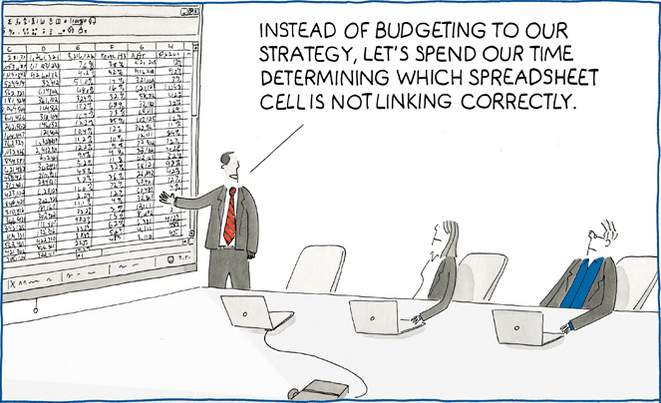
\includegraphics{images/spreadsheet_hell.png}
\caption{spreadsheet hell}
\end{figure}

*Image courtesy of \href{https://www.hive9.com/blog/just-say-no-to-spreadsheets}{hive9.com}

\hypertarget{the-grammar-of-tidy-data}{%
\section[The Grammar of Tidy Data]{\texorpdfstring{The Grammar of Tidy Data\footnote{Adapted from Hadley Wickham's paper on \href{https://vita.had.co.nz/papers/tidy-data.pdf}{Tidy Data}}}{The Grammar of Tidy Data}}\label{the-grammar-of-tidy-data}}

Democratic data analysis has an underlying structure, like a sentence. Rules exist so sentences (hopefully) make sense to you, the reader. Similarly, by following common conventions of democratic data analysis, others will be able to ``read'' your analysis like you are reading this sentence. And also, like grammar, you can and should break the rules-- but it helps to know them first.

Here are a couple definitions that will help as you move through this text. Don't worry about memorizing them, as I will refer back to these definitions frequently.

\hypertarget{fields}{%
\subsection{Fields}\label{fields}}

A field is a fancy name for a column.

From here on out, \textbf{every calculation, manipulation, formula, will be operated on a field}.

I want you to forget that you could ever modify a lonely cell in Excel. No more formulas in cells. No more typing in values to a cell. Certainly no more writing over data in a cell. And for the love of eveything that is good, no more color coding cells. Democratic data analysis depends on formulas that work on entire fields. Everything you would need to do to a single cell in Excel can-- and should!-- be done to an entire column. This may sound extreme and restrictive, but this approach will pay big dividends in your democratic data analysis journey and ultimately allow you to be more creative in your analysis.

\hypertarget{variables}{%
\subsection{Variables}\label{variables}}

A variable is something in your data that can change. That's it! Variables become very important when looking at how to structure your data. Each variable should have its own field (column).

\hypertarget{observations}{%
\subsection{Observations}\label{observations}}

Observations make up the rows of your data set. Each observation should correspond to a specific ``thing.'' This will make more sense later, I promise.

\hypertarget{values}{%
\subsection{Values}\label{values}}

Values are the actual data in your table.

Each value belongs to 1 (one) (uno) observation and 1 (one) variable. That's it.

This means, among other things, no more merged cells, merged rows, or groups. A one-to-one relationship between fields and observations is critical for getting the most out of your data analysis.

\hypertarget{tables}{%
\subsection{Tables}\label{tables}}

A table is the grouping of all observations of a similar type.

The table sets the foundation for analyzing your data. \textbf{If I could only convince you of one thing, it would be the value in keeping your data in a table-based excel format}. If you are trying to do math or statistics (again, not data anlysis. These things are different!), then the table based framework can sometimes fall short. But if you are concerned with working with data to draw conclusions, then tables are the way to go.

You may already be able to see how these definitions foreshadow some of what is coming in later sections. For example, there are no references to cells. This is intentional. The most important distinction between democratic data analysis and simply working in excel is that in democratic data analysis, (virtually) \emph{everything} is done on the \texttt{field} level. Changes are made to entire columns, calculations are made on entire columns. Thinking in \texttt{fields} is the first step on the path to democratic data enlightenment. Having data formatted in the structure outlined above forces good data hygiene that will be very helpful later on when discussing reproduciblity and pivot-ability.

\hypertarget{cleaning-and-tidying}{%
\section{Cleaning and Tidying}\label{cleaning-and-tidying}}

I hate cleaning, but love tidying. Unfortunately, as in with life, one must clean before one tidies. But let's start with some conceptual definitions.

Cleaning refers to the process of scrubbing the data into a way that makes sense to you, the analyst. Oftentimes, and especially in public sector organizations, the data is not clean. Whether you are looking at the output of a Survey Monkey survey or a canned report that is run from the IT department, your data will come in all shapes and sizes. Cleaning data is the process of transforming data values into ones that make sense for the purposes of your analysis.

Here is the first major departure from what you may have been taught about data analysis in Excel. When you get messy data \emph{do not} change individual cell values. Recall from the introductory chapter the difference between cells and fields. Fields, as a reminder, are columns that represent one variable. Use data analysis tools to make changes to the entire field, rather than specific cells.

Most data analysis software, outside of Excel, make it difficult or impossible to change individual cell values. At first glance, this can seem unnecessary, limiting, and supremely annoying. But it's actually very helpful. Thinking in terms of fields, and making changes to entire fields, will save you \emph{a lot} of work and headache in the long run.

Let's look at a sample dataset that may be similar to one you would encounter in real life. Here is a survey collected by a field manager of a local parks and recreation department on employment.

\begin{Shaded}
\begin{Highlighting}[]
\KeywordTok{library}\NormalTok{(tidyverse)}
\KeywordTok{library}\NormalTok{(DT)}

\NormalTok{sites <-}\StringTok{ }\KeywordTok{tribble}\NormalTok{(}
  \OperatorTok{~}\StringTok{"Employee"}\NormalTok{, }\OperatorTok{~}\StringTok{"Location"}\NormalTok{, }\OperatorTok{~}\StringTok{"Telecommute?"}\NormalTok{, }\OperatorTok{~}\StringTok{"Hire Date"}\NormalTok{,}
  \StringTok{"ron swanson"}\NormalTok{, }\StringTok{"Pawnee City Hall"}\NormalTok{, }\StringTok{"never"}\NormalTok{, }\StringTok{"Unknown"}\NormalTok{,}
  \StringTok{"Knope, Leslie"}\NormalTok{, }\StringTok{"Field Duty"}\NormalTok{, }\StringTok{"1 day/week"}\NormalTok{, }\StringTok{"2011-6-1"}\NormalTok{,}
  \StringTok{"Andy Dwyer"}\NormalTok{, }\StringTok{"sullivan street pit"}\NormalTok{, }\StringTok{"40 hours"}\NormalTok{, }\StringTok{"March 1, 2013"}\NormalTok{,}
  \StringTok{"Jerry Gergich"}\NormalTok{, }\StringTok{"City Hall"}\NormalTok{, }\StringTok{"never"}\NormalTok{, }\StringTok{"6/1/1985"}\NormalTok{,}
  \StringTok{"Garry Gergich"}\NormalTok{, }\StringTok{"City Hall"}\NormalTok{, }\StringTok{"never"}\NormalTok{, }\StringTok{"6/1/1985"}\NormalTok{,}
  \StringTok{"ben wyatt"}\NormalTok{, }\StringTok{"Partridge, Minnesota"}\NormalTok{,}\StringTok{""}\NormalTok{ , }\StringTok{"Jan. 1, 2010"}
\NormalTok{)}

\NormalTok{sites }\OperatorTok\StringTok{ }\KeywordTok{datatable}\NormalTok{(}
    \DataTypeTok{extensions =} \StringTok{'Buttons'}\NormalTok{, }
    \DataTypeTok{options =} \KeywordTok{list}\NormalTok{(}\DataTypeTok{dom =} \StringTok{'Bfrtip'}\NormalTok{, }
                   \DataTypeTok{buttons =} \StringTok{'excel'}\NormalTok{,}
                   \DataTypeTok{searching =} \OtherTok{FALSE}\NormalTok{))}
\end{Highlighting}
\end{Shaded}

\hypertarget{htmlwidget-6d669d781f234624c579}{}

In this example, it would be trivial to go in to the Excel file and clean up the dates, names, and locations by hand. However, you could imagine this survey replicated for a department of forty employees. It quickly becomes unfeasible to make those edits by hand. When this is the case, there are functions in Excel and R that will make your life much easier.

Here is annotated code for how I would go about cleaning this table in R. The friendly syntax of the \texttt{tidyverse} packages makes it easy to follow along, even if you aren't comfortable writing it yourself. You can accomplish all these similar transformations using \href{https://support.microsoft.com/en-us/office/power-query-101-008b3f46-5b14-4f8b-9a07-d3da689091b5}{Get \& Transform in Excel}.

\begin{Shaded}
\begin{Highlighting}[]
\CommentTok{#creating a new table called "sites_cleaned", starting with the old table "sites"}
\NormalTok{sites_cleaned <-}\StringTok{ }\NormalTok{sites }\OperatorTok\StringTok{ }
\StringTok{  }\CommentTok{#switching the order of names that are backwards}
\StringTok{  }\KeywordTok{mutate}\NormalTok{(}\DataTypeTok{Employee =} \KeywordTok{if_else}\NormalTok{(Employee }\OperatorTok{==}\StringTok{ "Knope, Leslie"}\NormalTok{, }\StringTok{"Leslie Knope"}\NormalTok{, Employee)) }\OperatorTok\StringTok{ }
\StringTok{  }\CommentTok{#seperate employee names into two columns}
\StringTok{  }\KeywordTok{separate}\NormalTok{(Employee, }\DataTypeTok{into =} \KeywordTok{c}\NormalTok{(}\StringTok{"first_name"}\NormalTok{, }\StringTok{"last_name"}\NormalTok{)) }\OperatorTok\StringTok{ }
\StringTok{  }\CommentTok{#renaming column names to standard format}
\StringTok{  }\KeywordTok{rename}\NormalTok{(}\DataTypeTok{location =}\NormalTok{ Location,}
         \DataTypeTok{telecommute_hours =}\StringTok{`}\DataTypeTok{Telecommute?}\StringTok{`}\NormalTok{,}
         \DataTypeTok{hire_date =} \StringTok{`}\DataTypeTok{Hire Date}\StringTok{`}\NormalTok{) }\OperatorTok\StringTok{ }
\StringTok{  }\CommentTok{#changing first and last names and locations to Title Case}
\StringTok{  }\KeywordTok{mutate}\NormalTok{(}\DataTypeTok{first_name =} \KeywordTok{str_to_title}\NormalTok{(first_name),}
         \DataTypeTok{last_name =} \KeywordTok{str_to_title}\NormalTok{(last_name),}
         \DataTypeTok{location =} \KeywordTok{str_to_title}\NormalTok{(location)) }\OperatorTok\StringTok{ }
\StringTok{  }\CommentTok{#coding location data to three categories, In Office, In Field, or Other}
\StringTok{  }\KeywordTok{mutate}\NormalTok{(}\DataTypeTok{location =} \KeywordTok{case_when}\NormalTok{(}
           \KeywordTok{str_detect}\NormalTok{(location, }\StringTok{"City Hall"}\NormalTok{) }\OperatorTok{~}\StringTok{ "In Office"}\NormalTok{,}
           \KeywordTok{str_detect}\NormalTok{(location, }\StringTok{"Field"}\NormalTok{) }\OperatorTok{~}\StringTok{ "In Field"}\NormalTok{,}
           \KeywordTok{str_detect}\NormalTok{(location, }\StringTok{"Street"}\NormalTok{) }\OperatorTok{~}\StringTok{ "In Field"}\NormalTok{,}
           \OtherTok{TRUE} \OperatorTok{~}\StringTok{ "Other"}\NormalTok{),}
  \CommentTok{#coding hours to numeric}
         \DataTypeTok{telecommute_hours =} \KeywordTok{case_when}\NormalTok{(}
\NormalTok{           telecommute_hours }\OperatorTok{==}\StringTok{ "never"} \OperatorTok{~}\StringTok{ }\DecValTok{0}\NormalTok{,}
\NormalTok{           telecommute_hours }\OperatorTok{==}\StringTok{ "1 day/week"} \OperatorTok{~}\StringTok{ }\DecValTok{8}\NormalTok{,}
\NormalTok{           telecommute_hours }\OperatorTok{==}\StringTok{ "40 hours"} \OperatorTok{~}\StringTok{ }\DecValTok{40}
\NormalTok{         )}
\NormalTok{         )}

\CommentTok{#print to datatable}
\NormalTok{sites_cleaned}\OperatorTok\StringTok{ }\KeywordTok{datatable}\NormalTok{(}
    \DataTypeTok{extensions =} \StringTok{'Buttons'}\NormalTok{, }
    \DataTypeTok{options =} \KeywordTok{list}\NormalTok{(}\DataTypeTok{dom =} \StringTok{'Bfrtip'}\NormalTok{, }
                   \DataTypeTok{buttons =} \StringTok{'excel'}\NormalTok{,}
                   \DataTypeTok{searching =} \OtherTok{FALSE}\NormalTok{))}
\end{Highlighting}
\end{Shaded}

\hypertarget{htmlwidget-1c45cfe6f2901a5e7e9e}{}

This may seem like a lot of work for a small table. But as your data grows, it is much easier to operate on entire fields at a time. This is especially true in Get \& Transform, which makes it very easy to transform and clean data using all the same steps as the \texttt{R} code above. As you can see, our table is now ``cleaned'' and organized consistently.

\hypertarget{tidying}{%
\section{Tidying}\label{tidying}}

Tidy data is the way your data should be organized before you begin your analysis. In tidy data, each column is a \emph{variable}, each row is an \emph{observation}, and each table is an \emph{associated set of observations}. What does that mean in practice? Consider the following example.

Below is a table\footnote{Data was created for demonstration purposes} that shows types of retirement visits for a month at a state's Department of Retirement Services by the employee who took the visit and the visit type.

\begin{Shaded}
\begin{Highlighting}[]
\CommentTok{#build sample data table}
\NormalTok{visits <-}\StringTok{ }\KeywordTok{tribble}\NormalTok{(}
  \OperatorTok{~}\StringTok{"Employee"}\NormalTok{, }\OperatorTok{~}\StringTok{"Phone Visits"}\NormalTok{, }\OperatorTok{~}\StringTok{"Office Visits"}\NormalTok{, }\OperatorTok{~}\StringTok{"Online Visits"}\NormalTok{,}
  \StringTok{"Danielle"}\NormalTok{, }\DecValTok{6}\NormalTok{, }\DecValTok{11}\NormalTok{, }\DecValTok{23}\NormalTok{,}
  \StringTok{"Ramona"}\NormalTok{, }\DecValTok{11}\NormalTok{, }\DecValTok{5}\NormalTok{, }\DecValTok{18}\NormalTok{,}
  \StringTok{"Ross"}\NormalTok{, }\DecValTok{10}\NormalTok{, }\DecValTok{10}\NormalTok{, }\DecValTok{10} 
\NormalTok{)}

\CommentTok{#print to datatable}
\NormalTok{visits}\OperatorTok\StringTok{ }\KeywordTok{datatable}\NormalTok{(}
    \DataTypeTok{extensions =} \StringTok{'Buttons'}\NormalTok{, }
    \DataTypeTok{options =} \KeywordTok{list}\NormalTok{(}\DataTypeTok{dom =} \StringTok{'Bfrtip'}\NormalTok{, }
                   \DataTypeTok{buttons =} \StringTok{'excel'}\NormalTok{,}
                   \DataTypeTok{searching =} \OtherTok{FALSE}\NormalTok{),}
                   \DataTypeTok{caption =} \StringTok{"Visits to the Dept. of Retirement Services in a given month by employee"}
\NormalTok{                   )}
\end{Highlighting}
\end{Shaded}

\hypertarget{htmlwidget-cb62e070176eb1ed9737}{}

Data are frequently displayed in this ``wide'' format. It works great for presentation, but not great for data analysis.

The shortcomings of data in this format may become apparent when you attempt to work with the data in a pivot table. This is because our columns aren't truly variables. Remember, variables are elements of an observation that can change. You can drag the fields from the top row to the grey box below, for columns, and the left, for rows. This becomes unmanageable quickly.

\begin{Shaded}
\begin{Highlighting}[]
\NormalTok{rpivotTable}\OperatorTok{::}\KeywordTok{rpivotTable}\NormalTok{(visits, }\DataTypeTok{width =} \StringTok{"60%"}\NormalTok{, }\DataTypeTok{height =} \StringTok{"60%"}\NormalTok{)}
\end{Highlighting}
\end{Shaded}

\hypertarget{htmlwidget-4770e46f7048113660e7}{}

\hypertarget{tidy-data--from-wide-to-long}{%
\section{Tidy Data- From Wide to Long}\label{tidy-data--from-wide-to-long}}

Let's apply our criteria of tidy data to this set:

\begin{itemize}
\tightlist
\item
  Variables

  \begin{itemize}
  \tightlist
  \item
    At first glance, it doesn't look like this is a problem. But think again. Is \texttt{phone\ visits} really a variable? Or is the real variable of interest number of visits? And are our column names are actually variables too (type of visit)?
  \end{itemize}
\end{itemize}

Let's take another swing at setting up our table for data analysis purposes. This can be accomplished easily in R using the code below, or in Excel by loading the data with \href{https://support.microsoft.com/en-us/office/unpivot-columns-power-query-0f7bad4b-9ea1-49c1-9d95-f588221c7098}{\texttt{Get\ and\ Transform}} -\textgreater{} selecting the three ``visits'' columns -\textgreater{} right clicking -\textgreater{} and selecting ``unpivot columns.''

\begin{Shaded}
\begin{Highlighting}[]
\CommentTok{#We have already loaded the "tidyverse" library so we do not have to do it again}
\CommentTok{#we are editing the "visits" table already created by storing it in a new table pivot_visits}
\NormalTok{pivot_visits <-}\StringTok{ }\NormalTok{visits }\OperatorTok\StringTok{ }
\StringTok{  }\CommentTok{#using pivot_longer on every column except "employee" and setting the name of the new columns}
\StringTok{  }\KeywordTok{pivot_longer}\NormalTok{(}\OperatorTok{-}\NormalTok{Employee, }\DataTypeTok{names_to =} \StringTok{"Visit Type"}\NormalTok{, }\DataTypeTok{values_to =} \StringTok{"Number of Visits"}\NormalTok{) }


\NormalTok{knitr}\OperatorTok{::}\KeywordTok{kable}\NormalTok{(pivot_visits, }\DataTypeTok{caption =} \StringTok{"Visits to the Dept. of Retirement Services in a given month"}\NormalTok{)}
\end{Highlighting}
\end{Shaded}

\begin{table}

\caption{\label{tab:unnamed-chunk-3}Visits to the Dept. of Retirement Services in a given month}
\centering
\begin{tabular}[t]{l|l|r}
\hline
Employee & Visit Type & Number of Visits\\
\hline
Danielle & Phone Visits & 6\\
\hline
Danielle & Office Visits & 11\\
\hline
Danielle & Online Visits & 23\\
\hline
Ramona & Phone Visits & 11\\
\hline
Ramona & Office Visits & 5\\
\hline
Ramona & Online Visits & 18\\
\hline
Ross & Phone Visits & 10\\
\hline
Ross & Office Visits & 10\\
\hline
Ross & Online Visits & 10\\
\hline
\end{tabular}
\end{table}

Now this is a table that is much easier to analyze in an Excel pivot table or with a variety of R functions. However, it does look worse and is less intuitive for human readers. Thankfully, using data in this format, it is easy to recreate the original table for presentation, while also giving a variety of options for formatting and plotting. Use the pivot table below to recreate the original table using the tidy data. *Hint- Instead of Count, select Sum -\textgreater{} Number of Visits as the value field. It is far easier to work with fields when they are in a tidy format.

\hypertarget{using-lower-level-data}{%
\section{Using lower level data}\label{using-lower-level-data}}

Let's introduce a slightly more complicated tidy data problem, using the same base data as before.

\begin{Shaded}
\begin{Highlighting}[]
\NormalTok{visits_retirements <-}\StringTok{ }\KeywordTok{tribble}\NormalTok{(}
  \OperatorTok{~}\StringTok{"Employee"}\NormalTok{, }\OperatorTok{~}\StringTok{"Phone Visits"}\NormalTok{, }\OperatorTok{~}\StringTok{"Phone Retirements"}\NormalTok{, }\OperatorTok{~}\StringTok{"Office Visits"}\NormalTok{, }\OperatorTok{~}\StringTok{"Office Retirements"}\NormalTok{, }\OperatorTok{~}\StringTok{"Online Visits"}\NormalTok{, }\OperatorTok{~}\StringTok{"Online Retirements"}\NormalTok{,}
  \StringTok{"Danielle"}\NormalTok{, }\DecValTok{6}\NormalTok{, }\DecValTok{4}\NormalTok{, }\DecValTok{11}\NormalTok{, }\DecValTok{8}\NormalTok{, }\DecValTok{23}\NormalTok{, }\DecValTok{15}\NormalTok{,}
  \StringTok{"Ramona"}\NormalTok{, }\DecValTok{11}\NormalTok{, }\DecValTok{7}\NormalTok{, }\DecValTok{5}\NormalTok{, }\DecValTok{3}\NormalTok{, }\DecValTok{18}\NormalTok{, }\DecValTok{15}\NormalTok{,}
  \StringTok{"Ross"}\NormalTok{, }\DecValTok{10}\NormalTok{, }\DecValTok{8}\NormalTok{, }\DecValTok{10}\NormalTok{, }\DecValTok{7}\NormalTok{, }\DecValTok{10}\NormalTok{, }\DecValTok{9} 
\NormalTok{)}

\NormalTok{knitr}\OperatorTok{::}\KeywordTok{kable}\NormalTok{(visits_retirements, }\DataTypeTok{caption =} \StringTok{"Visits to the Dept. of Retirement Services in a given month by employee and associated client retirements"}\NormalTok{)}
\end{Highlighting}
\end{Shaded}

\begin{table}

\caption{\label{tab:unnamed-chunk-4}Visits to the Dept. of Retirement Services in a given month by employee and associated client retirements}
\centering
\begin{tabular}[t]{l|r|r|r|r|r|r}
\hline
Employee & Phone Visits & Phone Retirements & Office Visits & Office Retirements & Online Visits & Online Retirements\\
\hline
Danielle & 6 & 4 & 11 & 8 & 23 & 15\\
\hline
Ramona & 11 & 7 & 5 & 3 & 18 & 15\\
\hline
Ross & 10 & 8 & 10 & 7 & 10 & 9\\
\hline
\end{tabular}
\end{table}

Hopefully you will see a similar pattern here. Now, there are three variables: Visit type, number of visits, and number of retirements. Again, this data works fine for presentation but could use tidying to ease in analysis.

\begin{Shaded}
\begin{Highlighting}[]
\NormalTok{visits_retirements }\OperatorTok
\StringTok{  }\NormalTok{DT}\OperatorTok{::}\KeywordTok{datatable}\NormalTok{(}
    \DataTypeTok{extensions =} \StringTok{'Buttons'}\NormalTok{, }
    \DataTypeTok{options =} \KeywordTok{list}\NormalTok{(}\DataTypeTok{dom =} \StringTok{'Bfrtip'}\NormalTok{, }
                   \DataTypeTok{buttons =} \StringTok{'excel'}\NormalTok{,}
                   \DataTypeTok{searching =} \OtherTok{FALSE}\NormalTok{))}
\end{Highlighting}
\end{Shaded}

\hypertarget{htmlwidget-2a48ffe3848219e5b4b5}{}

Try to tidy this in R or Excel Get and Transform. See this footnote\footnote{powerquery hints} or look at the code if you need a hint.

\begin{Shaded}
\begin{Highlighting}[]
\NormalTok{visits_retirements_tidy <-}\StringTok{ }\NormalTok{visits_retirements }\OperatorTok
\StringTok{  }\KeywordTok{pivot_longer}\NormalTok{(}\DataTypeTok{cols =} \OperatorTok{-}\NormalTok{Employee, }
               \DataTypeTok{names_to =} \KeywordTok{c}\NormalTok{(}\StringTok{"Visit Location"}\NormalTok{, }\StringTok{"Type"}\NormalTok{), }
               \DataTypeTok{names_sep =} \StringTok{" "}\NormalTok{)}

\KeywordTok{print}\NormalTok{(visits_retirements_tidy)}
\end{Highlighting}
\end{Shaded}

\begin{verbatim}
## # A tibble: 18 x 4
##    Employee `Visit Location` Type        value
##    <chr>    <chr>            <chr>       <dbl>
##  1 Danielle Phone            Visits          6
##  2 Danielle Phone            Retirements     4
##  3 Danielle Office           Visits         11
##  4 Danielle Office           Retirements     8
##  5 Danielle Online           Visits         23
##  6 Danielle Online           Retirements    15
##  7 Ramona   Phone            Visits         11
##  8 Ramona   Phone            Retirements     7
##  9 Ramona   Office           Visits          5
## 10 Ramona   Office           Retirements     3
## 11 Ramona   Online           Visits         18
## 12 Ramona   Online           Retirements    15
## 13 Ross     Phone            Visits         10
## 14 Ross     Phone            Retirements     8
## 15 Ross     Office           Visits         10
## 16 Ross     Office           Retirements     7
## 17 Ross     Online           Visits         10
## 18 Ross     Online           Retirements     9
\end{verbatim}

In this case, we actually pivoted too far. It will probably be more useful to have the counts of visits and retirements in their own category. Keep in mind the scope of the observation-- It is perfectly valid for each to have their own column, as it is visits and retirements per month.

\begin{Shaded}
\begin{Highlighting}[]
\NormalTok{visits_retirements_tidy2 <-}\StringTok{ }\NormalTok{visits_retirements_tidy }\OperatorTok\StringTok{ }
\StringTok{  }\KeywordTok{pivot_wider}\NormalTok{(}\DataTypeTok{id_cols =} \KeywordTok{c}\NormalTok{(Employee, }\StringTok{`}\DataTypeTok{Visit Location}\StringTok{`}\NormalTok{, Type), }\DataTypeTok{names_from =}\NormalTok{ Type, }\DataTypeTok{values_from =}\NormalTok{ value)}

\KeywordTok{print}\NormalTok{(visits_retirements_tidy2)}
\end{Highlighting}
\end{Shaded}

\begin{verbatim}
## # A tibble: 9 x 4
##   Employee `Visit Location` Visits Retirements
##   <chr>    <chr>             <dbl>       <dbl>
## 1 Danielle Phone                 6           4
## 2 Danielle Office               11           8
## 3 Danielle Online               23          15
## 4 Ramona   Phone                11           7
## 5 Ramona   Office                5           3
## 6 Ramona   Online               18          15
## 7 Ross     Phone                10           8
## 8 Ross     Office               10           7
## 9 Ross     Online               10           9
\end{verbatim}

From here, it is easy to do calculations based on fields, rather than cells. For example, in R or Get and Transform, you could add the following:

\begin{Shaded}
\begin{Highlighting}[]
\NormalTok{visits_pct <-}\StringTok{ }\NormalTok{visits_retirements_tidy2 }\OperatorTok\StringTok{ }
\StringTok{  }\KeywordTok{mutate}\NormalTok{(}\DataTypeTok{pct_retirements =}\NormalTok{ Retirements }\OperatorTok{/}\StringTok{ }\NormalTok{Visits)}

\KeywordTok{print}\NormalTok{(visits_pct)}
\end{Highlighting}
\end{Shaded}

\begin{verbatim}
## # A tibble: 9 x 5
##   Employee `Visit Location` Visits Retirements pct_retirements
##   <chr>    <chr>             <dbl>       <dbl>           <dbl>
## 1 Danielle Phone                 6           4           0.667
## 2 Danielle Office               11           8           0.727
## 3 Danielle Online               23          15           0.652
## 4 Ramona   Phone                11           7           0.636
## 5 Ramona   Office                5           3           0.6  
## 6 Ramona   Online               18          15           0.833
## 7 Ross     Phone                10           8           0.8  
## 8 Ross     Office               10           7           0.7  
## 9 Ross     Online               10           9           0.9
\end{verbatim}

And then, one of the most useful things you can do is develop formulas by grouping of rows. For example, you may want to know the total number of visits and retirements by retiree, regardless of visit location. That can be accomplished in a pivot table, which we will cover in the next section.

\hypertarget{how-is-this-democratic}{%
\section{How is this democratic?}\label{how-is-this-democratic}}

Thinking of your analysis in terms of tidy data is the first step on your way to democratic data analysis.

\hypertarget{conclusion}{%
\section{Conclusion}\label{conclusion}}

\hypertarget{practicesresources}{%
\section{Practices/Resources}\label{practicesresources}}

\hypertarget{pivot-to-win-it}{%
\chapter{Pivot to Win It}\label{pivot-to-win-it}}

\begin{quote}
\emph{Has anyone in this family ever even seen a pivot table?} - Michael Bluth
\end{quote}

Why did we go through all the trouble of tidying data in the last section? So we can pivot. Thinking in terms of pivots, aka fields and summaries, is the key to effective democratic data analysis

\hypertarget{pivot-tables-and-the-meaning-of-everything}{%
\section{Pivot Tables and the Meaning of Everything}\label{pivot-tables-and-the-meaning-of-everything}}

Pivot tables are the world's most common, most helpful, and most underrated data analysis tool. If you understand the mechanics of the pivot table, you have everything you need to be a data analysis expert. PowerBI or Tableau interactive charts and graphs are just pivot tables in disguise. Understanding what is needed to make a pivot table work is the key to the wide world of data analysis.

What is so important about pivot tables? First and foremost, pivot tables force you to think in terms of fields, not in terms of cells. In order for a pivot table to be effective, the data has to be organized in a table. And there is a right and a wrong way to putting data in a table. If your pivot table is not working properly, it is likely because your data isn't tidy.

A pivot table groups data by field and allows the user to drag fields to the rows or columns of the pivot table. This is effective when each field is a variable (something that can change), and each row is a separate observation of some phenomena of interest.

In short, pivot tables depend on \textbf{tidy data}.

Recall our sample data from the last chapter:

\begin{Shaded}
\begin{Highlighting}[]
\CommentTok{#We have already loaded the "tidyverse" library so we do not have to do it again}
\CommentTok{#we are editing the "visits" table already created by storing it in a new table pivot_visits}
\NormalTok{pivot_visits <-}\StringTok{ }\NormalTok{visits }\OperatorTok\StringTok{ }
\StringTok{  }\CommentTok{#using pivot_longer on every column except "employee" and setting the name of the new columns}
\StringTok{  }\KeywordTok{pivot_longer}\NormalTok{(}\OperatorTok{-}\NormalTok{Employee, }\DataTypeTok{names_to =} \StringTok{"Visit Type"}\NormalTok{, }\DataTypeTok{values_to =} \StringTok{"Number of Visits"}\NormalTok{) }


\NormalTok{knitr}\OperatorTok{::}\KeywordTok{kable}\NormalTok{(pivot_visits, }\DataTypeTok{caption =} \StringTok{"Visits to the Dept. of Retirement Services in a given month"}\NormalTok{)}
\end{Highlighting}
\end{Shaded}

\begin{table}

\caption{\label{tab:unnamed-chunk-9}Visits to the Dept. of Retirement Services in a given month}
\centering
\begin{tabular}[t]{l|l|r}
\hline
Employee & Visit Type & Number of Visits\\
\hline
Danielle & Phone Visits & 6\\
\hline
Danielle & Office Visits & 11\\
\hline
Danielle & Online Visits & 23\\
\hline
Ramona & Phone Visits & 11\\
\hline
Ramona & Office Visits & 5\\
\hline
Ramona & Online Visits & 18\\
\hline
Ross & Phone Visits & 10\\
\hline
Ross & Office Visits & 10\\
\hline
Ross & Online Visits & 10\\
\hline
\end{tabular}
\end{table}

Once the data has been tidied, it is easy to manipulate fields in pivot tables.

\begin{Shaded}
\begin{Highlighting}[]
\NormalTok{rpivotTable}\OperatorTok{::}\KeywordTok{rpivotTable}\NormalTok{(pivot_visits, }\DataTypeTok{width =} \StringTok{"60%"}\NormalTok{, }\DataTypeTok{height =} \StringTok{"400px"}\NormalTok{)}
\end{Highlighting}
\end{Shaded}

\hypertarget{htmlwidget-0b8106dfc7e01e6fff53}{}

The key with pivot tables, such as the one above, is you are moving \emph{fields} into the rows and columns of a new table. This is often referred to as ``pivoting''. You are then selecting a calculation to \emph{summarize} the intersection of the \emph{fields} that you drug into rows and columns. Above, you can click on the ``Count'' button to see the other ways this lightweight pivot table allows you to \emph{summarize} your data. More powerful data analysis tools, such as PowerPivot in Excel, PowerBI, and several R packages allow you infinitely flexible formulas to define what happens at the intersection of fields in a pivot table. This is the core of all (most) data analysis. Think in terms of fields and calculated summaries and you are well on your way to becoming a democratic data master.

It is also easier to do a variety of calculations on the data now that is in a ``tidy'' format. For example, creating descriptive statistics across groups is very straightforward. This can also be accomplished in an Excel pivot table with the basic \href{https://support.microsoft.com/en-gb/office/show-different-calculations-in-pivottable-value-fields-014d2777-baaf-480b-a32b-98431f48bfec}{``show values as'' functions}.

\begin{Shaded}
\begin{Highlighting}[]
\NormalTok{desc_visits <-}\StringTok{ }\NormalTok{pivot_visits }\OperatorTok\StringTok{ }
\StringTok{  }\KeywordTok{group_by}\NormalTok{(}\StringTok{`}\DataTypeTok{Visit Type}\StringTok{`}\NormalTok{) }\OperatorTok\StringTok{ }
\StringTok{  }\KeywordTok{summarise}\NormalTok{(}\StringTok{`}\DataTypeTok{Avg Visits}\StringTok{`}\NormalTok{ =}\StringTok{ }\KeywordTok{mean}\NormalTok{(}\StringTok{`}\DataTypeTok{Number of Visits}\StringTok{`}\NormalTok{),}
            \StringTok{`}\DataTypeTok{Total Visits}\StringTok{`}\NormalTok{ =}\StringTok{ }\KeywordTok{sum}\NormalTok{(}\StringTok{`}\DataTypeTok{Number of Visits}\StringTok{`}\NormalTok{),}
            \StringTok{`}\DataTypeTok{Std Dev of Visits}\StringTok{`}\NormalTok{ =}\StringTok{ }\KeywordTok{sd}\NormalTok{(}\StringTok{`}\DataTypeTok{Number of Visits}\StringTok{`}\NormalTok{))}
\end{Highlighting}
\end{Shaded}

This is where pivot tables, and the way they force you to think about data, become \emph{enormously} powerful. Enter \textbf{PowerPivot}, stage left. PowerPivot allows you to write very detailed and useful functions for the values that appear in the middle of a pivot table. Above, I used R to calculate the average number of visits, total visits, and standard deviation of visits by visit type. But what if I quickly wanted to view this by Employee instead? Or what if I wanted to group by both visit type and employee, and generate the same descriptions? R and PowerPivot make this very easy. I'm not going to go into detail on the mechanics and tutorials of PowerPivot, as it is extensively covered elsewhere-- see the Practices section of this guide.

Here's the key-- Every fancy data dashboard, analysis technique, interactive visualization-- is a pivot table with a ``calculated field'' (formula for values in a pivot table). That's it. If you can think in terms of fields and calculated values based on those fields, PowerBI, PowerPivot, Tableau, Qlik, ggplot2, etc. will be second nature. The only thing that changes when crating a viz instead of a pivot table is that your fields that you drag into a pivot table become the axis of your chart, and your calculated field becomes a ``mark'' on your plot. If you are interested more in a universal so-called ``grammar of graphics'' that is based on the principles outlined here, there is a wealth of resources available. (link to resources.)

\hypertarget{advanced-data-summaries}{%
\section{Advanced Data Summaries}\label{advanced-data-summaries}}

Frequently, public administrators are interested in how things have changed over a period of time. Here's an example dataset that shows referrals to the same Dept. of Retirement Systems we have used in previous examples.

\hypertarget{conclusion-1}{%
\section{Conclusion}\label{conclusion-1}}

Thinking in terms of pivot tables is the core of democratic data analysis. This may not feel intuitive at first glance. But thinking this way forces the analyst to avoid the classic pitfalls of \emph{un}democratic data analysis. Those pitfalls are the cell-based, hard-coded, pages and pages of tabs excel workbook nightmare that only the analyst themselves understands (and that's if they are lucky). Thinking in terms of the language of data analysis, emphasizing the use of fields and summaries, forces your analysis to be flexible, understandable, and reproducible. It is easy for an analyst who is also fluent in data analysis to pick up your work and immediately see how it operates because it is constructed using best practices and principles. It is also easy for someone else, or your future self, to write new calculations for data summaries, compare results, and use different fields.

\hypertarget{practices}{%
\section{Practices}\label{practices}}

\hypertarget{reproducible-analysis}{%
\chapter{Reproducible Analysis}\label{reproducible-analysis}}

\begin{quote}
\emph{``And that's why you always leave a note.''} --- J. Walter Weatherman
\end{quote}

\hypertarget{do-it-for-your-future-self}{%
\section{Do It For Your Future Self}\label{do-it-for-your-future-self}}

Many things take more time to do up front, but save you from massive headaches down the road. Brushing your teeth. Oil changes. Preventative maintenance is the name of the game. The same thing applies in democratic data analysis. Learning how to brush the teeth of your analysis will pay massive dividends down the road, as someone else (or you, more likely), need to go back through and understand, replicate, or validate your findings.

The second principle of democratic data analysis is reproducability. By this, I mean anything that makes it easy to look at your analysis and understand what is going on. This is where classic data analysis in Excel falls short. I believe it is almost a universal experience in the public sector to receive a workbook full of broken links, formulas pointing in every direction, and no sense of where the original data is or what has happened to it since.

In thinking about creating reproducible data analysis, it is important to keep in mind that data analysis should be structured from beginning to end, like a story. In the beginning, there is raw data that you pulled from a report, compiled yourself, or otherwise received. In Act 1, you use the practices we learned in the previous section to make the raw data tidy-- without destroying the original data. You should use tools that allow to to non-destructively manipulate and iterate on your data. Both Get \& Transform and R allow you to do this by default. In Act 2, which will be the next chapter, you use your data to create a picture of the world before you share it with others in the final Act 3.

The practices of reproducability that you will use here apply throughout the other chapters. It may seem like a waste of time, but if you have ever come back to a complicated excel workbook after spending even days away, this will make your life much easier.

\hypertarget{do-not-destroy}{%
\subsection{Do Not Destroy}\label{do-not-destroy}}

As I mentioned before, the existential dread that occurs when opening someone else's workbook and immediately receiving broken links, color-coding\footnote{for the love of democracy, PLEASE do not color code your data}, and a spiderweb of formulas may be a universal experience in the public sector. But there is a better way to do things. Reproducible analysis is linear. It progresses in a certain direction-- from data load to final analysis. Things happen discretely. The blessing and curse of spreadsheets is that they are unbound by time. There is no natural direction, just a sea of little boxes spreading out as far as the eye can see\footnote{This is where programming languages such as R have an inherent advantage. Code runs in order, from first to last}. However, there are ways to impose a linear structure to your analysis.

The first thing I want to emphasize is PLEASE DO NOT DESTROY, ALTER, OR MANIPULATE YOUR UNDERLYING DATA. Your underlying data is like the foundation of your house. Democratic data analysis starts with a foundation of data, and builds on top of it. Oftentimes, it seems easier to simply click and drag cells around in an excel workbook, changing values here and there as you see fit. This may work in small use cases, but what if you have another idea? Or come up with a different question, where your data needs to be coded differently? Reproducible analysis makes it substantially easier to revise and rewrite after the fact. If you were writing a well-sourced research article, you wouldn't delete your notes and references for the material that didn't make it into your final product. In the same way, keeping record of the changes that you make to your analysis will pay dividends when your approach changes.

\hypertarget{red-flags-for-reproducibility}{%
\subsection{Red flags for reproducibility}\label{red-flags-for-reproducibility}}

I'll start with a list of things you want to avoid in the pursuit of reproducible democratic data analysis

\hypertarget{copy-and-paste}{%
\subsubsection{Copy and Paste}\label{copy-and-paste}}

If you find yourself copying and pasting values in an excel workbook, you are not engaging in reproducible analysis-- full stop. Copy and paste (or worse, cut and paste) doesn't leave breadcrumbs for you or anyone who may come after you. It is incredibly difficult to follow the trail of an analysis built on top of copy-paste.

\hypertarget{repeating-yourself}{%
\subsubsection{Repeating Yourself}\label{repeating-yourself}}

There is an old adage in programming - \emph{D}on't \emph{R}epeat \emph{Y}ourself. DRY. Keeping your data analysis DRY is a good habit to get in to. If you find yourself repeating the same task more than three times, chances are there is a better, more programmatic way to go about what you are doing.

What do I mean by repeating yourself? This would be going through every row of an 100-row table to add (or remove)a space between words, capitalizing letters, doing specific calculations. All of these tasks can be \textbf{easily} automated using virtually all data analysis tools. This not only saves you time, but makes it easier for your reader to see how the data has changed in the course of your analysis.

To preview the Practices section, Get and Transform allows you to make flexible value transformations on entire fields at a time. This reduces the need for repetitive data cleaning. And if you are already taking my advice and no longer editing individual data cells, you will have a much easier time avoiding repeating yourself.

\hypertarget{comment-everything}{%
\section{Comment Everything}\label{comment-everything}}

Comments are wonderful. They are notes to yourself that you should leave at almost every step of your analysis. I frequently do not leave comments. Never have I come back to an uncommented data transformation and been happy with my past self. At worst, leaving comments takes a couple seconds of your time you will never get back. At best, it saves you or your organization from a massive headache when you are able to catch your own errors or update your analysis easier in the future.

\hypertarget{give-yourself-credit}{%
\section{Give Yourself Credit}\label{give-yourself-credit}}

Don't hard code (e.g.~manually type) Excel values in cells. Build calculated summaries as discussed in the pivot-powered tab. Link to data sources. Highlight your expertise. This is easier to do when you use the tools shown in the practices section.

\hypertarget{version-control}{%
\section{Version Control}\label{version-control}}

\hypertarget{save-as}{%
\subsection{Save as}\label{save-as}}

\hypertarget{gitgithub}{%
\subsection{Git/GitHub}\label{gitgithub}}

If you are inclined to use R or another programming language for data analysis (and you really should be) then git is an essential tool in your toolkit. Full disclosure, even I am not an expert on it. But there are several tools available to make version control using git seamless and effortless.

Git is an automated version control system that backs up your changes to the cloud, typically to github.com or another similar provider. It is very cool. For example, you can examine all the source code for this very book on \href{https://github.com/nemethc/dataisfordemocracy/tree/master/doingdemocraticdataanalysis}{GitHub}.

\hypertarget{practices-1}{%
\section{Practices}\label{practices-1}}

The value of Get \& Transform Data is that it forces you to build on top of your data foundation. It also conveniently records each step along the way. You even have the ability to save comments right there in the query editor. This is a remarkably easy and intuitive way to build a data transformation pipeline that will be valuable know and into the future.

\href{https://www.bitss.org/opa/}{The Berkeley Open Policy Analysis Initiative}

\href{https://www.bitss.org/wp-content/uploads/2019/03/OPA-Guidelines.pdf}{Open Policy Analysis Guidelines}

\hypertarget{uncertainty-oriented-analysis}{%
\chapter{Uncertainty Oriented Analysis}\label{uncertainty-oriented-analysis}}

\begin{quote}
\emph{``I mean its one banana Michael. What could it cost, \$10?''}- Lucille Bluth
\end{quote}

\begin{quote}
\emph{All models are wrong, but some are useful}-- George Box
\end{quote}

\begin{quote}
\emph{A person with a watch knows what time it is. A man with two watches is never sure}- Segal's Law
\end{quote}

\hypertarget{embracing-uncertainty-for-better-outcomes}{%
\section{Embracing Uncertainty for Better Outcomes}\label{embracing-uncertainty-for-better-outcomes}}

What is the point of data analysis? Often, it is to use data to summarize the world around you. In a sense, all data analysis is model building, and by definition, a model is a simplified version of the world. Any time the analyst is using data analysis to inform decision making, she is in a sense making a model. Models are commonly thought of to provide answers to the question at hand. Model building, and data analysis more generally, never gives you ``the'' answer. Data analysis only gives you a answer, if it gives you an answer at all. If you have been following along to this point, you have learned the value of data analysis that is structured and built up, not out. Frequently, data analysis is valuable because it tells you what isn't the answer. As in the quote above, knowing the difference between the watches tells you something important. One watch doesn't tell you what you don't know\^{}{[}adapted from {[}Statistical Modeling, by Daniel T Kaplan{]}(\url{https://dtkaplan.github.io/SM2-bookdown/introduction.html}. Knowing how to build uncertainty into your analysis is incredibly valuable as analysis -- models-- are used to implement important policies that impact the public good. Incorporating uncertainty into your analysis will make you both more credible and force you to use your subject matter expertise in addition to your data skills.

\hypertarget{what-is-a-model}{%
\section{What is a Model?}\label{what-is-a-model}}

A model is anything that is used to represent the world. By definition, anything that represents the world simplifies it, becuase the world is vastly complex. An average value of a dataset is a model. Same with the median, mode, and the other so-called \emph{descriptive statistics} that you may be familiar with.

When you create a data model, you bring all your expertise, subjectivity, and creativity to the table. Data modeling can

Models transform data into decision making. Models are useful exactly because they are wrong! Because models are wrong, we can critically examine the wrong-ness of them to inform decisionmaking in a way that embraces uncertainty.

\hypertarget{examples-of-models-in-the-public-sector}{%
\section{Examples of Models in the Public Sector}\label{examples-of-models-in-the-public-sector}}

\hypertarget{incorporating-uncertainty-into-models}{%
\section{Incorporating Uncertainty Into Models}\label{incorporating-uncertainty-into-models}}

\hypertarget{example-two}{%
\section{Example two}\label{example-two}}

\begin{figure}
\centering
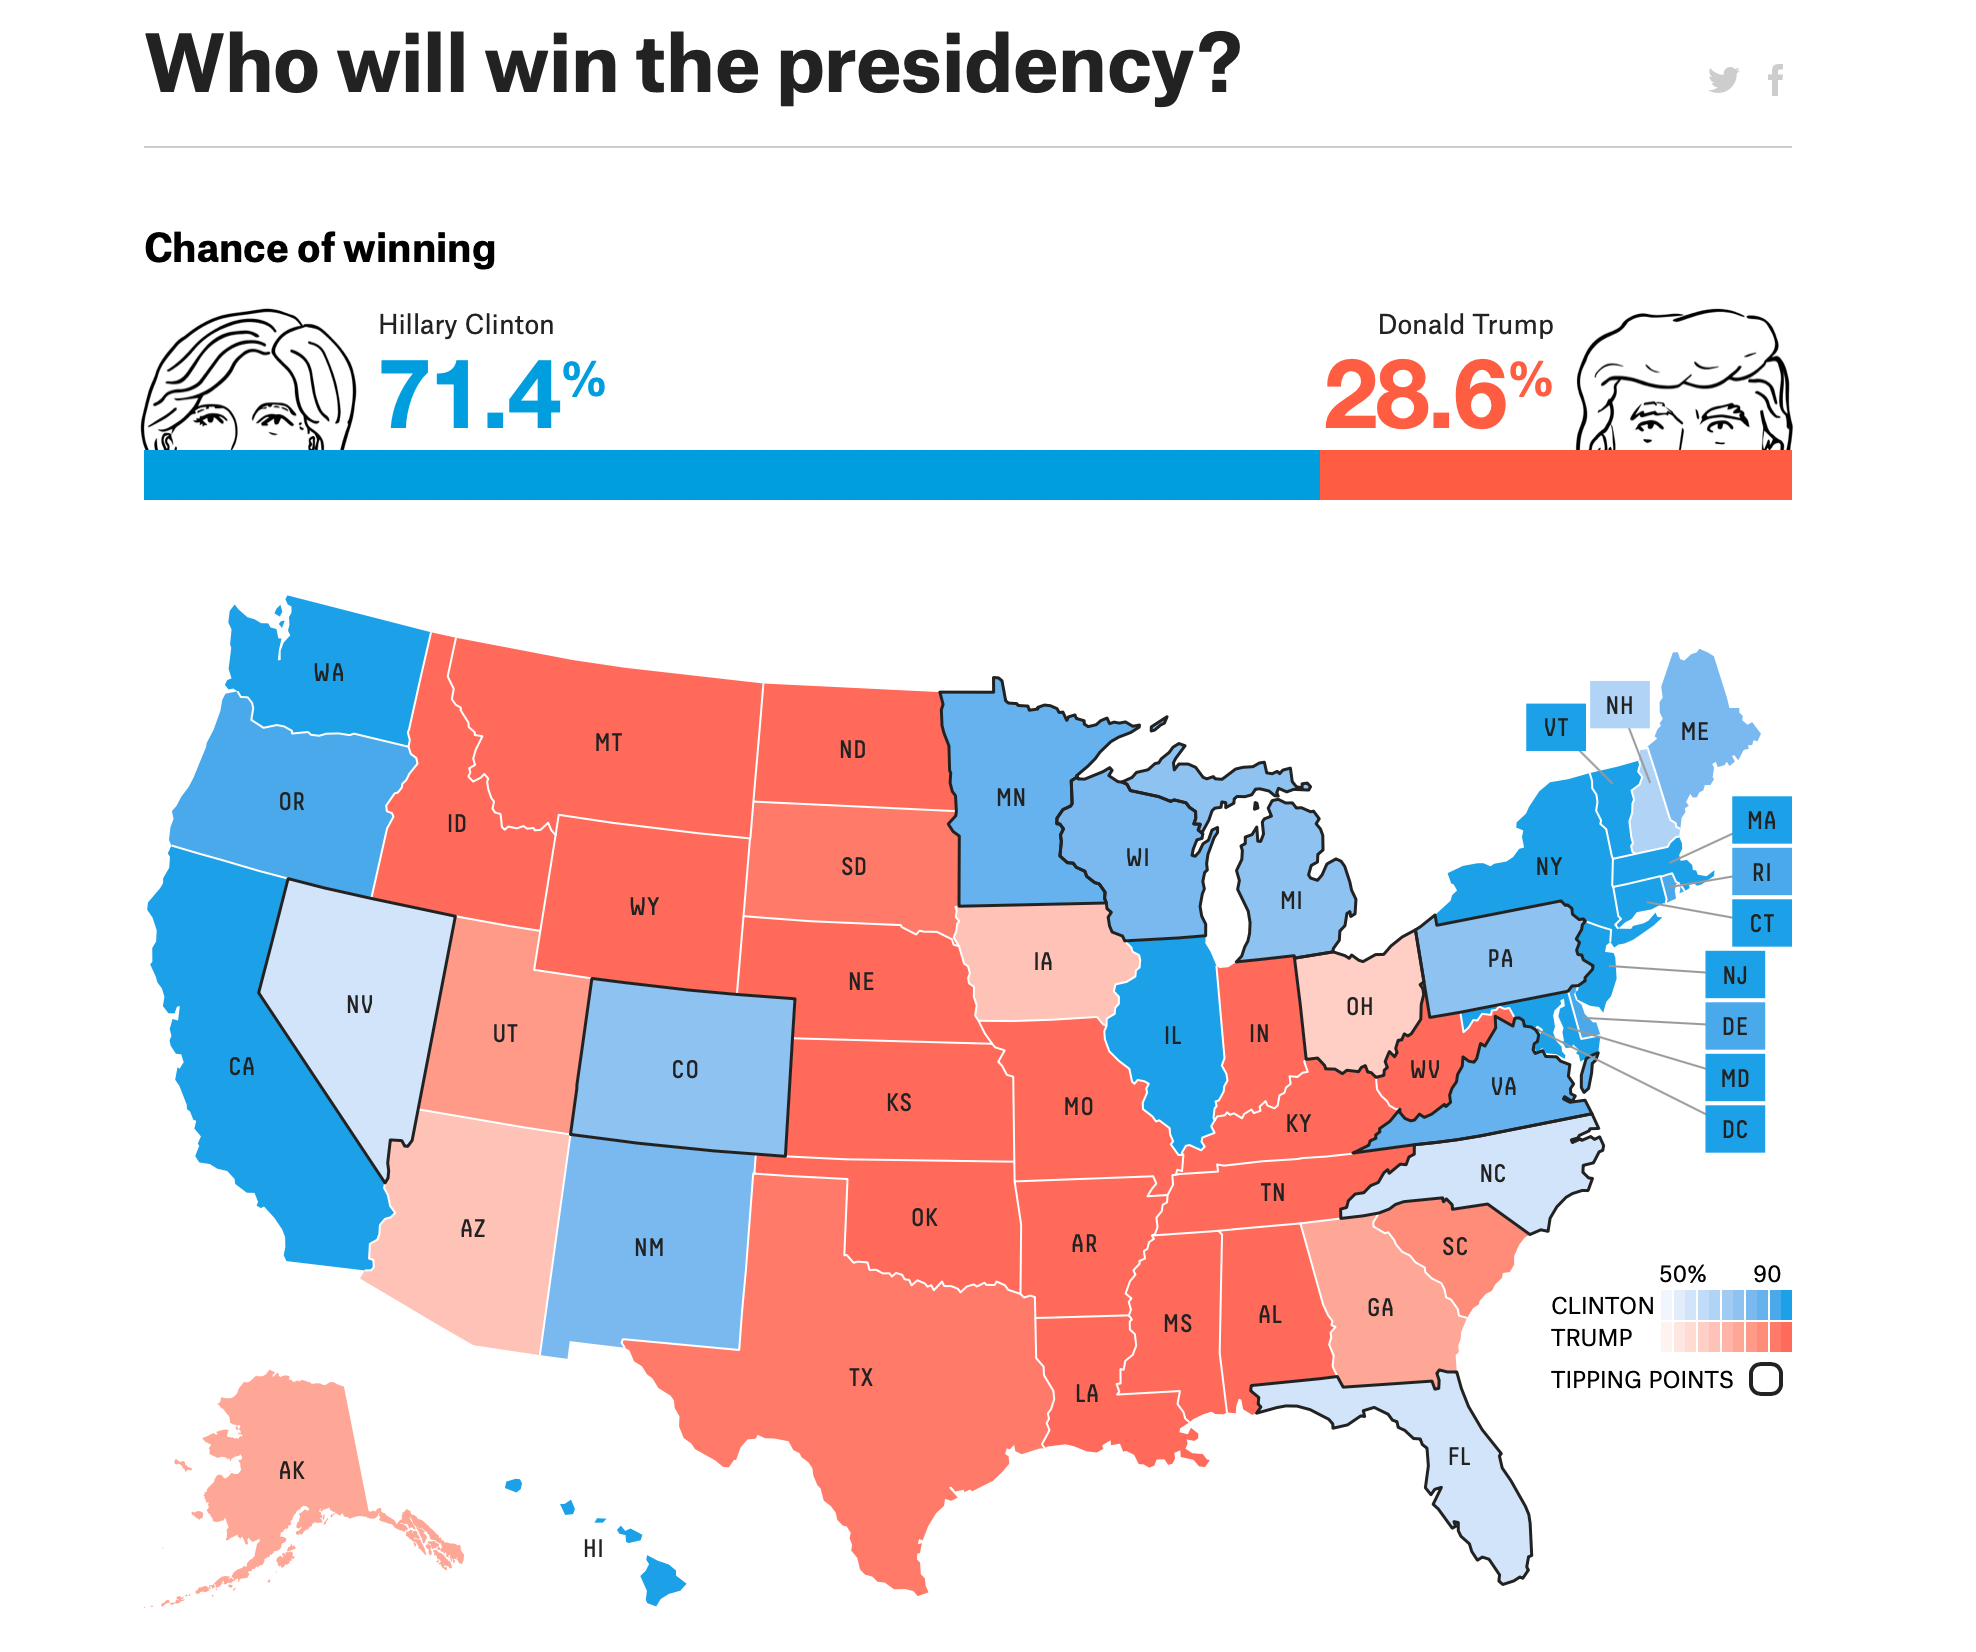
\includegraphics{images/map.png}
\caption{electoral 2016 map}
\end{figure}

\begin{figure}
\centering
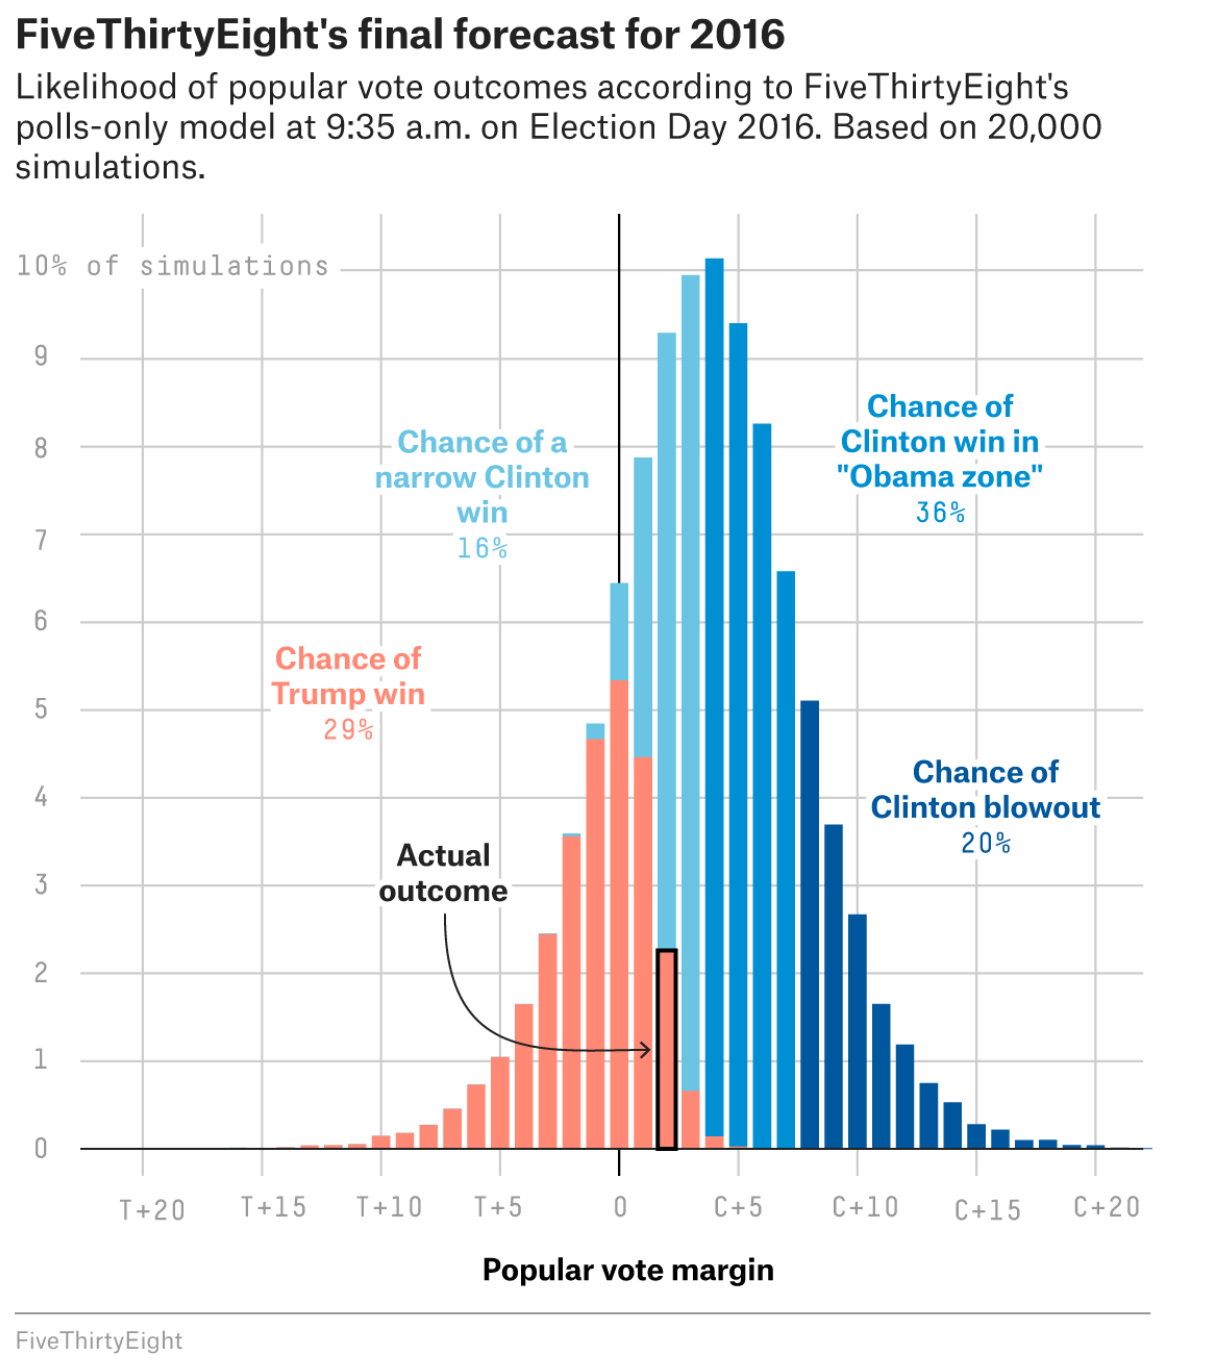
\includegraphics{images/uncertain_dist.png}
\caption{distribution of possible results}
\end{figure}

\hypertarget{use-assumptions-and-document-them}{%
\section{Use Assumptions, and Document Them}\label{use-assumptions-and-document-them}}

By clearly documenting your assumptions, you allow them to vary as your understanding changes.

\hypertarget{practices-2}{%
\section{Practices}\label{practices-2}}

Talk about modeling implies math or statistics, when it really doesn't. All a model seeks to do is to simply phenomena in a manner that can be comprehended and used to make decisions in conjunction with subject matter expertise.

\hypertarget{audience-focused}{%
\chapter{Audience-Focused}\label{audience-focused}}

\begin{quote}
Theres always money in the banana stand - George Bluth
\end{quote}

Just like writing, your data analysis always has an audience. Whether the audience is you, your coworker, your boss, or a policymaker, knowing your audience helps tailor how you present your findings.

\hypertarget{the-audience-is-you}{%
\section{The audience is you}\label{the-audience-is-you}}

This is where your reproducible principles are key. Because you are likely to forget that you edited cell B7, did a few copy/pastes, and hard-coded over some values when you come back to your workbook in a few weeks (or days, for that matter).

\hypertarget{the-audience-is-a-peer}{%
\section{The audience is a peer}\label{the-audience-is-a-peer}}

\hypertarget{the-audience-is-your-manager}{%
\section{The audience is your manager}\label{the-audience-is-your-manager}}

\hypertarget{show-and-tell--use-highlights-and-captions.-design-your-data-visualization.-please-god-dont-use-the-defaults}{%
\section{Show and Tell- Use highlights and captions. Design your data visualization. Please god don't use the defaults}\label{show-and-tell--use-highlights-and-captions.-design-your-data-visualization.-please-god-dont-use-the-defaults}}

Sometimes a table is totally appropriate. Sometimes it isn't.

What is the message you are trying to convey? There is no such thing as a neutral visualization.

Text is a data visualization. How can you bundle your data analysis and explanatory text?
Designed excel workbooks as backup
Rmarkdown/notebook format-- the future.
Interactive documents
Classic papers with accompanying backup.

\#\#Visualization is anything that presents your evidence-- think critically about it!

\hypertarget{the-audience-is-a-policydecision-maker}{%
\section{The audience is a policy/decision maker}\label{the-audience-is-a-policydecision-maker}}

When sharing data analysis with a policymaker or decision maker, it is important to keep in mind that the audience will often be much wider than initially assumed. Once your analysis is in the hands of a policymaker, it may go to the press, lobbyist organizations, other interest groups, or others inside or outside your organization. Additionally, policymakers often prefer paper or other ``hard copy'' type analysis, limiting your flexibility to simply share a file. This poses two unique constraints:

\begin{enumerate}
\def\labelenumi{\arabic{enumi})}
\tightlist
\item
  The mechanics of your analysis are often hidden in a print or a PDF
\item
  Others will see your work and either take it for granted or want to dissect it.
\end{enumerate}

This is where having tidy, reproducible, and flexible backup becomes incredibly important. By having this backup ready to go as soon as you present or deliver your analysis to the policymaker, you are putting yourself in a strong position to share backup when questions inevitably arise.

If you are sharing your work electronically, then there are several emerging technologies and techniques that make this process easier. It is possible to embed Excel workbooks within Word documents, which ensures that the recipient has access to both your analysis and your methods. However, this can be tricky for ensuring adequate version control and reproducible, as these workbooks will often link to data that the end user doesn't have access to.

This problem is largely solved by using dashboards and other online solutions. Dashboards are an effective way to share analysis with decision makers because you can present your conclusions and also offer the tailored flexibility for the end user to interact as well. Tools such as PowerBI and Tableau run on the same tidy data and pivot-oriented platform discussed here. It is also straightforward to share the mechanics of the model with anyone who is interested-- especially if you follow the best practices for reproducibility outlined earlier. The downside of such dashboard solutions is they can be expensive, proprietary, and it can be difficult to configure them for specific audiences.

\hypertarget{my-audience-is-all-of-the-above--an-introduction-to-literate-data-analysis}{%
\section{My audience is all of the above- An Introduction to Literate Data Analysis}\label{my-audience-is-all-of-the-above--an-introduction-to-literate-data-analysis}}

That brings me to what form democratic data analysis would take in the World-According-To-Corban. Another tool for presenting data analysis to decision-makers are interactive notebooks that merge explanatory text, data, code, and graphics in one file that can be tailored for a variety of audiences. I call this approach \textbf{\emph{literate data analysis}}\footnote{derived from Literate Programming, but specific to subject matter expert data analysis}. Code-and-text driven notebooks are becoming exceedingly common in academic domains. In fact, this handbook is an example of an interactive HTML document written in \texttt{r}\footnote{using Rmarkdown files and the \href{bookdown.org}{bookdown} package}, but they certainly do not have to be this involved. Interactive notebooks combine text, code, and output in one place. They can be structured so that the file shows either plain-text analysis and charts in a web browser, but all of the code that generates it if you open the file in an editor such as RStudio. For example, \href{https://nemethc.com/evaluating_legislator_efficiency.nb.html\#}{here is an R notebook that I authored for a research project on legislative voting behavior}, and I'll link to other interactive notebooks in the Practices section.

Here are three platforms of interactive, code-driven data analysis notebooks:

\begin{itemize}
\tightlist
\item
  \href{https://rmarkdown.rstudio.com}{Rmarkdown notebooks}
\item
  \href{https://jupyter-notebook.readthedocs.io/en/stable/}{Jupyter notebooks}
\item
  \href{https://observablehq.com}{Observable notebooks}
\end{itemize}

I firmly believe that the notebook approach is the future of policy and data analysis in the public sector. These tools are free, robust, and accessible to those with varying levels of technical expertise. They also inherently solve the challenges of reproducible data analysis that I have been examining here. Version-controlled interactive notebooks are flexible, shareable, editable, and allow both decision-makers and analysts to use the same file to either draw conclusions or validate results.

I dream of a future when budgetary fiscal notes, quantitative bill analysis, and data models in the public sector are written as interactive notebooks, with explanatory text and analysis bundled together, version controlled, and presented with assumptions clearly documented.

This isn't to say that there aren't downsides to these approaches. The largest, as it currently stands, is the learning curve required to use these tools. I have yet to come across a notebook format that is as easily intuitive as an Excel workbook\footnote{\href{https://beta.grid.is/@grid/what-is-grid-yBYeOyirSSKBlknj25F98A}{Grid} looks promising, but I haven't had a chance to full look into it yet}. For now, the biggest downside of these tools is that they require at least a baseline understanding of \texttt{r}, \texttt{python}, \texttt{javascript}, or another similar scripting language. As we have already covered, Excel is a programming language, and probably the world's most common one at that. But Excel is familiar and relatively beginner friendly because it hides the fact that the user is actually programming.

Once that baseline level of understanding is acquired, the notebook format becomes an intuitive output for reports. The same document can result in a PDF file to be shared with decision makers, an interactive document to be shared online, and a complete record of your analysis for a peer. Long story short, I'm excited to work towards integrating the notebook philosophy to the public sector as the next frontier of democratic data analysis.

Yihui Xie, the creator of Rmarkdown, summarizes these principles nicely:
\textgreater{} I think notebooks are popular for the same reason that explains the popularity of spreadsheets such as Excel. I haven't met a single software engineer who loves Excel. Everyone hates it and makes fun of it, but why do so many users still use it? Again, Excel makes things tangible. You can touch the data (although it is usually a very bad idea), and draw graphics in a sheet that contains the source data (bad idea again). It makes you feel everything is well under your control: oh here is my data, and here is a graph next to it; oh I should use that column to draw the graph instead, so let me change it and I can see the updated graph immediately.2 You can do everything in a single place, and the short distance between the source (data) and the output is ace.

\begin{quote}
Excel makes things tangible at the price of making things messy (e.g., it may contain manually edited data that is hard to keep track of, or merged cells or graphs that make it hard for other software to read the data). By comparison, although notebooks can mess up the state, but that is only an intermediate problem. At its core, it is still relatively clean and encourages the reproducibility principle, i.e., you shall use code to generate results automatically instead of manually copying and pasting results in your report. If you are concerned about the state, you can restart the session and recompile the whole notebook from scratch. Spreadsheets are often hopeless here---you cannot easily restart your brain and redo exactly the same things.
\end{quote}

-Yihui Xie, Creator of Rmarkdown on \href{https://yihui.org/en/2018/09/notebook-war/}{notebooks and excel}

\hypertarget{applications-and-resources}{%
\chapter{Applications and Resources}\label{applications-and-resources}}

\begin{quote}
``I hear the jury's still out on science.'' - Gob Bluth

``There are dozens of us. Dozens!'' - Tobias Fünke
\end{quote}

\hypertarget{tying-it-all-together}{%
\section{Tying it all together}\label{tying-it-all-together}}

How does this play out in the real world?

Questions to ask yourself:
How can I pivot off of this data?

How can I think in terms of fields?

How can I make this more democratic?

\hypertarget{situations-and-examples}{%
\section{Situations and Examples}\label{situations-and-examples}}

\hypertarget{fiscal-analyis}{%
\subsection{Fiscal Analyis}\label{fiscal-analyis}}

Fiscal notes-- quantifying uncertainty and employing reproducibility

\hypertarget{policy-analysis}{%
\subsection{Policy Analysis}\label{policy-analysis}}

Saez and Zucman open policy analysis of Warren proposals

\hypertarget{budget-analysis}{%
\subsection{Budget Analysis}\label{budget-analysis}}

\hypertarget{surveys-and-samples}{%
\subsection{Surveys and Samples}\label{surveys-and-samples}}

\hypertarget{additional-resources}{%
\section{Additional Resources}\label{additional-resources}}

\hypertarget{r}{%
\subsection{R}\label{r}}

\begin{itemize}
\tightlist
\item
  \href{https://r4ds.had.co.nz/}{R for Data Science}
\item
  \href{https://learn.r-journalism.com/en/}{R for Journalism}
\item
  \href{https://bbc.github.io/rcookbook/}{BBC Journalism Guide to R Graphics}
\item
  Graphing in R- \href{https://rstudio.com/wp-content/uploads/2015/03/ggplot2-cheatsheet.pdf}{ggplot2 cheat sheet}, \href{https://serialmentor.com/dataviz/}{Fundamentals of Data Visualization}
\item
  Interactive Documents in R- \href{https://bookdown.org/yihui/rmarkdown/}{Guide to Rmarkdown}; \emph{learn how to make books and reports like this one!}
\item
  Data Wrangling in R- \href{https://dplyr.tidyverse.org/}{dplyr} for manipulation and \href{https://github.com/tyleransom/EconometricsLabs/blob/master/tidyRcheatsheet.pdf}{tidyr} for tidying
\end{itemize}

\hypertarget{excel}{%
\subsection{Excel}\label{excel}}

\begin{itemize}
\tightlist
\item
  \href{https://support.office.com/en-us/article/get-started-with-power-pivot-in-microsoft-excel-fdfcf944-7876-424a-8437-1a6c1043a80b}{Getting Started with PowerPivot}
\item
  \href{https://www.tandfonline.com/doi/full/10.1080/00031305.2017.1375989}{Principles for Data Organization in Spreadsheets}
\item
  I am not the only one saying these things, \href{https://towardsdatascience.com/microsoft-excel-in-the-era-of-big-data-401e67ca28a5}{promise!}
\item
  \href{https://powerpivotpro.com/2015/10/giving-back-steal-this-reference-card/\#downloads}{Power Pivot Quick Reference Card}
\end{itemize}

\hypertarget{reproduciblity}{%
\subsection{Reproduciblity}\label{reproduciblity}}

\begin{itemize}
\tightlist
\item
  \href{https://ropensci.org}{ROpenSci}
\item
  \href{https://github.com/ukgovdatascience}{UK Government Data Science repository}
\item
  I really promise I'm not the only one-- \href{https://www.bitss.org/opa/}{The Berkeley Open Policy Analysis Initiative}

  \begin{itemize}
  \tightlist
  \item
    \href{https://www.bitss.org/wp-content/uploads/2019/03/OPA-Guidelines.pdf}{Open Policy Analysis Guidelines}
  \end{itemize}
\end{itemize}

\hypertarget{examples-of-democratic-data-analysis-in-the-wild}{%
\subsection{Examples of Democratic Data Analysis in the Wild}\label{examples-of-democratic-data-analysis-in-the-wild}}

\begin{itemize}
\item
  \href{http://wealthtaxsimulator.org/analysis/}{Dynamic Documentation for Senator Warren's Wealth Tax Policy Analysis}
\item
  \href{https://arstechnica.com/tech-policy/2018/11/how-i-changed-the-law-with-a-github-pull-request/}{Using version control to change laws}
\item
  {[}UK publishing official government statistics with Rmarkdown\}(\url{https://blog.revolutionanalytics.com/2017/03/uk-statistics.html})

  \begin{itemize}
  \tightlist
  \item
    \href{https://ukgovdatascience.github.io/govdown/}{Template}
  \end{itemize}
\item
\item
\end{itemize}

\bibliography{book.bib,packages.bib}

\end{document}
